\section{Resultados}
\label{sec:resultados}

% Os resultados devem ser apresentados de forma clara e objetiva. Gráficos,
% tabelas e figuras podem ser utilizados para melhor visualização dos dados
% obtidos.

Esta seção apresenta os resultados obtidos com a implementação do método
\textit{Smoothed Particle Hydrodynamics} (SPH) utilizando a arquitetura
\textit{Entity Component System} (ECS). Inicialmente, são apresentadas as
configurações de hardware, software e os parâmetros utilizados nos
experimentos. Em seguida, é analisado o desempenho da implementação em função
da quantidade de partículas, considerando a taxa de quadros por segundo e o
tempo de processamento de cada passo da simulação.

\subsection{Configuração da simulação}
\label{subsec:simulation_setup}

Os experimentos foram realizados utilizando uma simulação bidimensional baseada
em partículas SPH. Cada partícula representa uma pequena porção do fluido e
armazena propriedades físicas locais utilizadas durante os cálculos de
densidade, pressão e viscosidade.

A implementação foi desenvolvida e executada em um notebook Acer Predator
Helios Neo 16S AI. A Tabela~\ref{tab:hardware_specs} apresenta a configuração
de hardware e software utilizada durante os experimentos.

\begin{table}[H]
\centering
\caption{Configuração do ambiente utilizado nos experimentos.}
\label{tab:hardware_specs}
\begin{tabular}{l l}
\hline
Componente & Especificação \\
\hline
Sistema operacional & CachyOS Linux x86\_64 \\
Kernel & Linux 7.0.10 \\
Processador & Intel Core Ultra 9 275HX \\
Quantidade de núcleos & 24 núcleos, 24 threads \\
Frequência máxima & 5.40 GHz \\
GPU dedicada & NVIDIA GeForce RTX 5070 Ti Mobile \\
GPU integrada & Intel Graphics \\
Memória RAM & 32 GB DDR5 6400MHz \\
\hline
\end{tabular}
\end{table}

Os experimentos foram realizados variando a quantidade de partículas entre 50 e
10,000. Os demais parâmetros foram mantidos constantes durante as execuções. A
Tabela~\ref{tab:simulation_parameters} apresenta os valores utilizados.

\begin{table}[H]
\centering
\caption{Parâmetros utilizados na simulação SPH.}
\label{tab:simulation_parameters}
\begin{tabular}{l c}
\hline
Parâmetro & Valor \\
\hline
Quantidade de partículas & 50--10000 \\
Tamanho de partícula & 2.0 \\
Raio de suporte (\(h\)) & 50.0 \\
Passo temporal (\(\Delta t\)) & 0.2 \\
Passos simulados (\(N_s\)) & 250 \\
Densidade alvo (\(\rho\)) & 0.000425 \\
Viscosidade (\(\nu\)) & 0.8 \\
Multiplicador de Pressão (\(-\nabla p/\rho\)) & 250.0 \\
Gravidade (\(g\)) & 1.0 \\
Resolução da simulação & \(1920 \times 1080\) \\
\hline
\end{tabular}
\end{table}

\subsection{Resultados visuais}
\label{subsec:visual_results}

As Figuras~\ref{fig:simulation_01} e~\ref{fig:simulation_02} apresentam
diferentes momentos da execução da simulação SPH. As imagens permitem
visualizar o comportamento das partículas durante a execução do programa,
evidenciando a formação e o deslocamento do fluido no ambiente de simulação.

\begin{figure*}[t]
\centering

\begin{subfigure}[b]{0.99\textwidth}
  \centering
  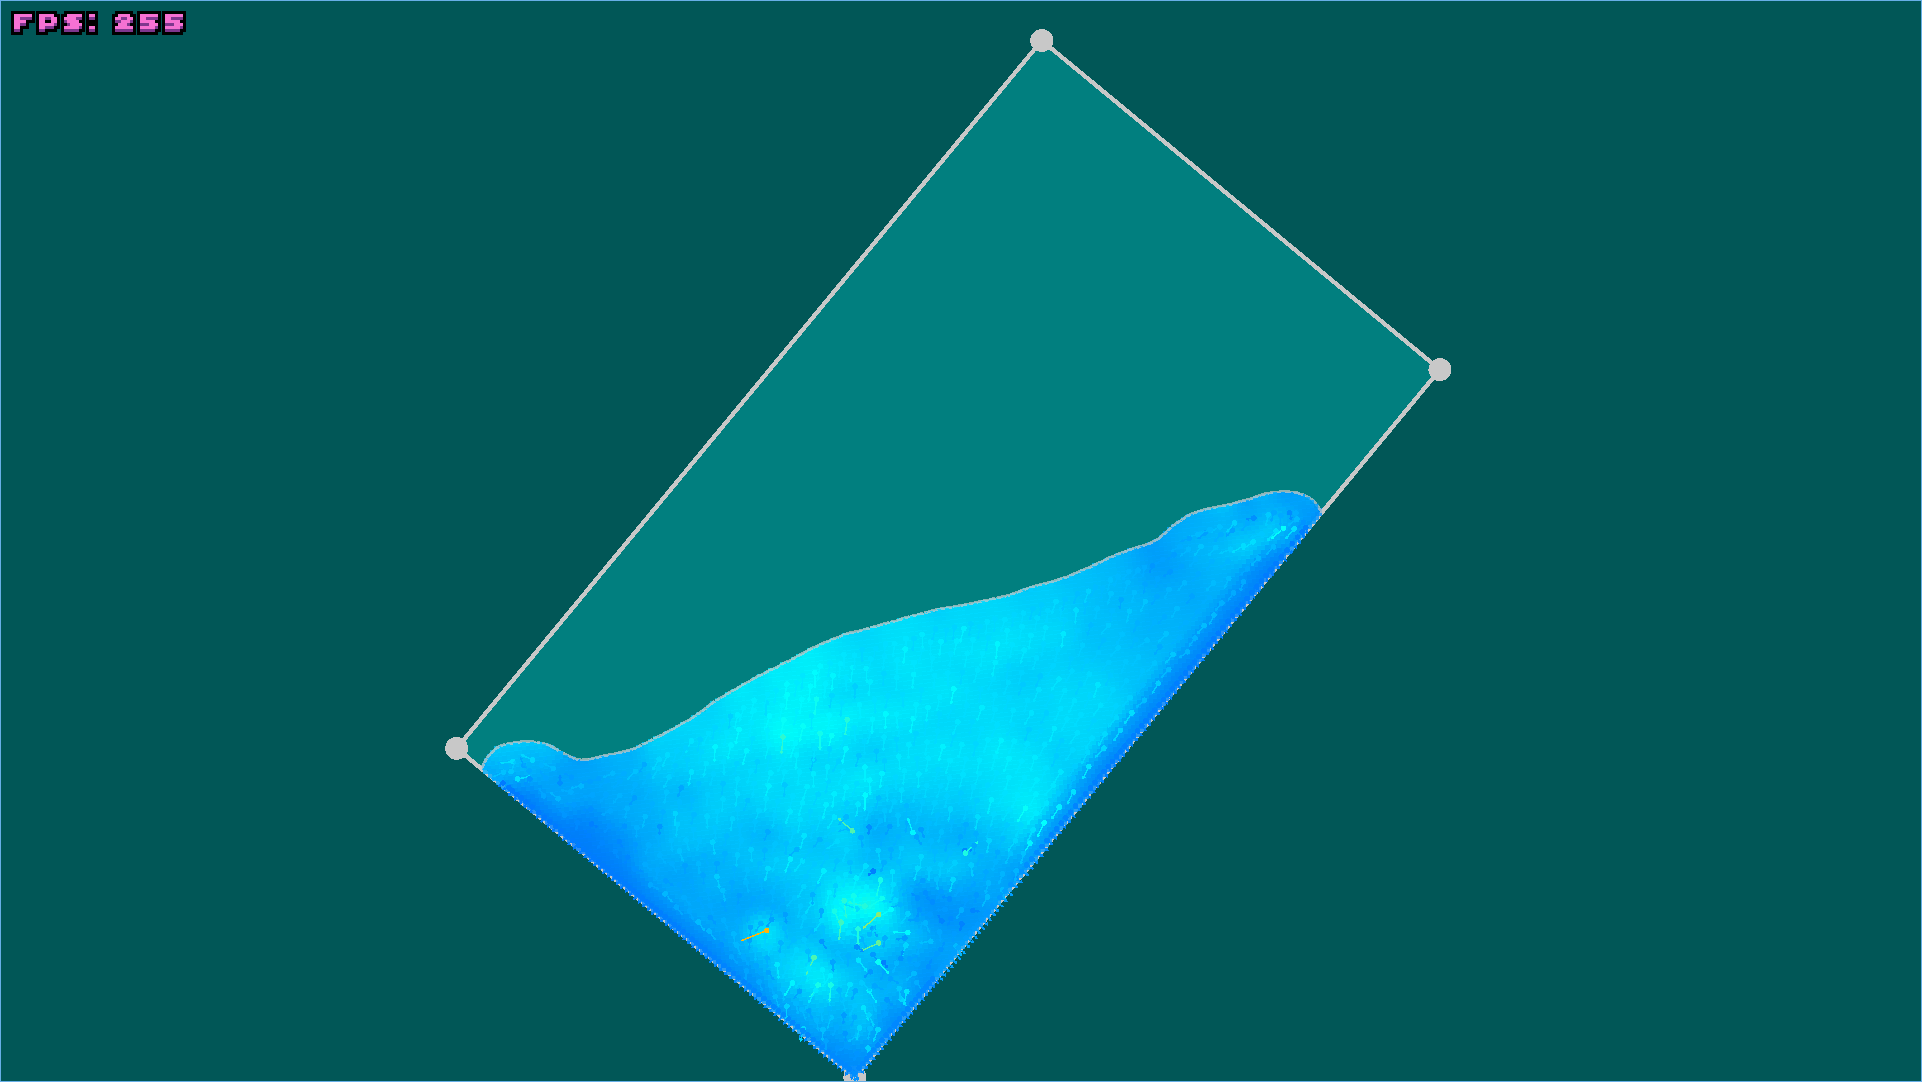
\includegraphics[width=\linewidth]{./fig/simulation_01.png}
  \caption{Primeiro momento da simulação.}
  \label{fig:simulation_01}
\end{subfigure}
\hfill
\begin{subfigure}[b]{0.99\textwidth}
  \centering
  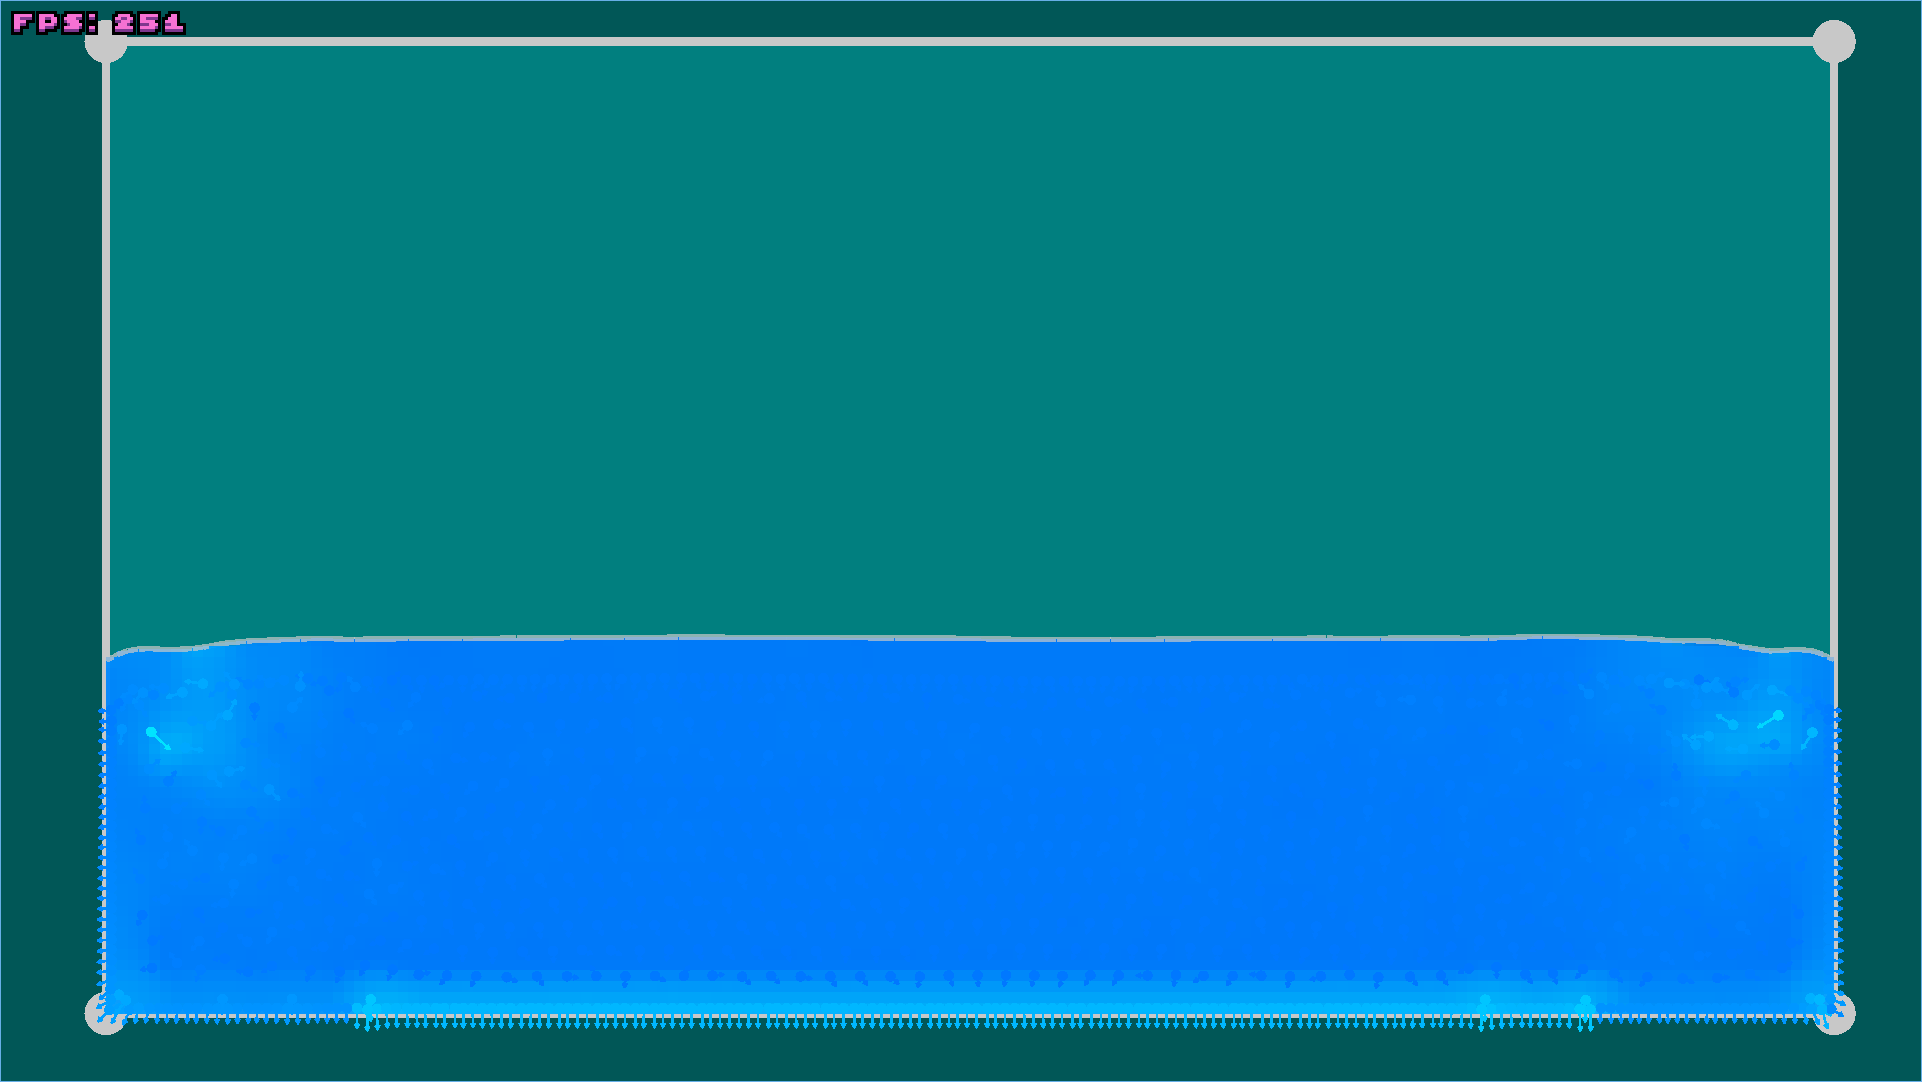
\includegraphics[width=\linewidth]{./fig/simulation_02.png}
  \caption{Segundo momento da simulação.}
  \label{fig:simulation_02}
\end{subfigure}

\caption{Diferentes momentos da execução da simulação SPH.}
\label{fig:simulation_running}
\end{figure*}

\subsection{Desempenho computacional}
\label{subsec:computational_performance}

O desempenho foi avaliado em duas configurações. A primeira corresponde à
execução \textit{headless}, na qual a simulação é executada sem a etapa de
renderização gráfica. A segunda corresponde à execução completa, incluindo a
renderização das partículas na resolução de (1920\times1080).

Essa distinção permite avaliar separadamente o custo associado ao processamento
da simulação e o custo adicional introduzido pela renderização. Nos gráficos
apresentados a seguir, a série representada em amarelo corresponde à execução
\textit{headless}, enquanto a série representada em vermelho corresponde à
execução com renderização.

\subsubsection{Taxa de quadros}

A Figura~\ref{fig:results_fps} apresenta a taxa de quadros por segundo (FPS) em
função da quantidade de partículas para as duas configurações de execução.

\begin{figure}[H]
\centering
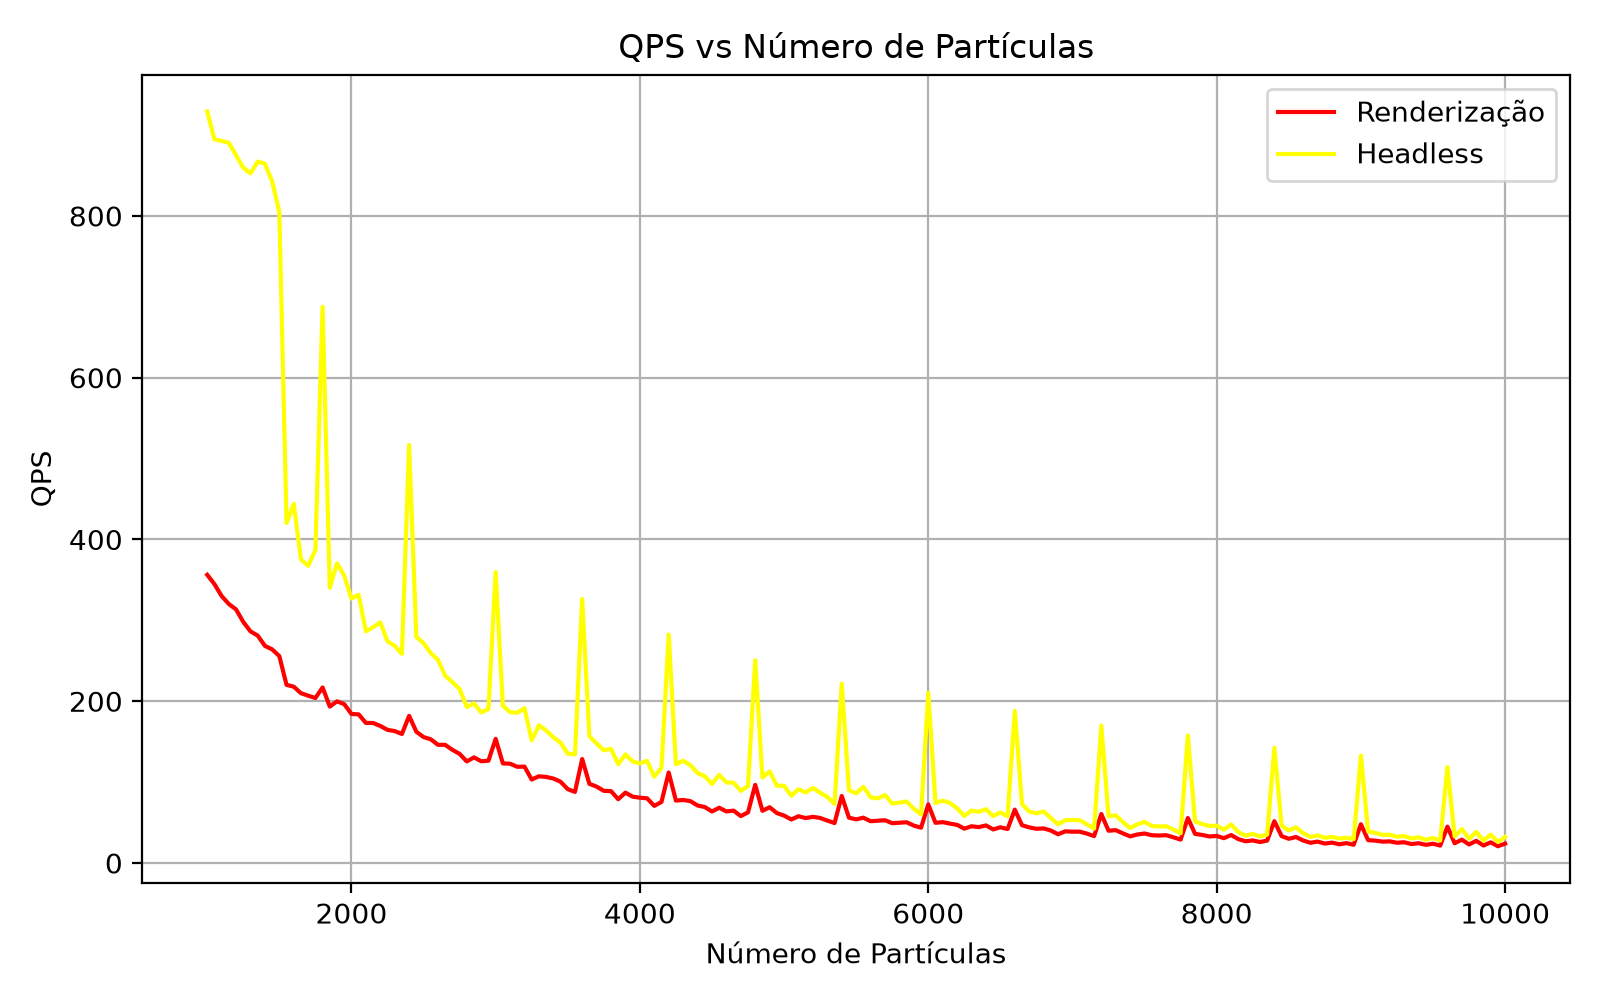
\includegraphics[width=0.49\textwidth]{./fig/results_fps.png}
\caption{Taxa de quadros por segundo em função da quantidade de partículas. A
  série amarela corresponde à execução \textit{headless} e a série vermelha à
  execução com renderização.}
\label{fig:results_fps}
\end{figure}

Em ambas as configurações, observa-se uma redução da taxa de quadros à medida
que a quantidade de partículas aumenta. Esse comportamento decorre do aumento
do número de operações necessárias para calcular as propriedades e interações
entre as partículas.

A execução \textit{headless} apresenta desempenho superior à execução com
renderização em toda a faixa avaliada. Para 10,000 partículas, por exemplo,
a execução \textit{headless} atingiu aproximadamente (32{,}2) FPS, enquanto
a execução com renderização atingiu aproximadamente (23{,}9) FPS. Portanto,
nessa configuração, a renderização introduziu um custo adicional perceptível
sobre o desempenho total da aplicação.

\subsubsection{Tempo de processamento}

A Figura~\ref{fig:results_time} apresenta o tempo médio necessário para
processar cada passo da simulação em função da quantidade de partículas.

\begin{figure}[H]
\centering
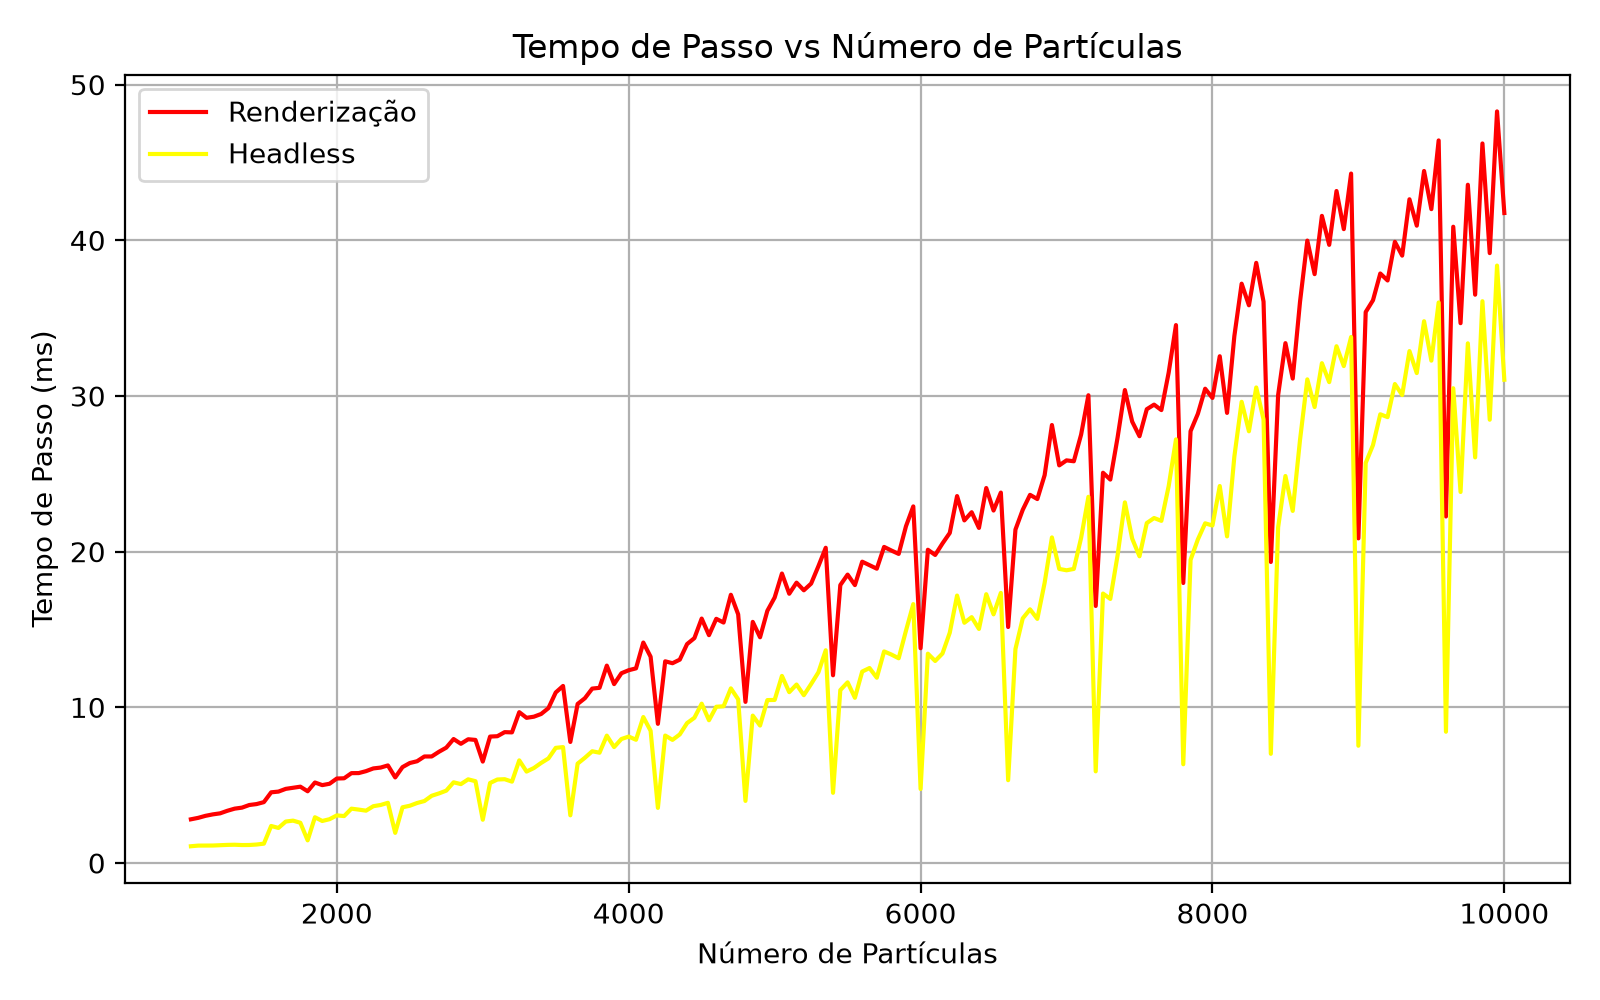
\includegraphics[width=0.49\textwidth]{./fig/results_time.png}
\caption{Tempo de processamento por passo em função da quantidade de
  partículas. A série amarela corresponde à execução \textit{headless} e a
  série vermelha à execução com renderização.}
\label{fig:results_time}
\end{figure}

Os resultados apresentam o comportamento inverso ao observado no gráfico de
FPS: o tempo necessário para executar cada passo aumenta com a quantidade de
partículas. Para 10,000 partículas, o tempo médio por passo foi de
aproximadamente (31{,}0) ms na execução \textit{headless} e (41{,}8) ms na
execução com renderização.

A diferença entre as duas configurações evidencia o impacto da renderização
sobre o tempo total de execução. Enquanto a versão \textit{headless} permite
avaliar predominantemente o custo computacional da simulação SPH, a versão com
renderização inclui também o processamento necessário para apresentar os
resultados graficamente.

Considerando os dois indicadores em conjunto, observa-se que o aumento da
quantidade de partículas reduz progressivamente o desempenho da aplicação.
Ainda assim, a versão com renderização mantém aproximadamente (24) FPS com
10,000 partículas, enquanto a versão \textit{headless} permanece acima de (30)
FPS nessa configuração.
